% Options for packages loaded elsewhere
\PassOptionsToPackage{unicode}{hyperref}
\PassOptionsToPackage{hyphens}{url}
%
\documentclass[
]{article}
\usepackage{lmodern}
\usepackage{amssymb,amsmath}
\usepackage{ifxetex,ifluatex}
\ifnum 0\ifxetex 1\fi\ifluatex 1\fi=0 % if pdftex
  \usepackage[T1]{fontenc}
  \usepackage[utf8]{inputenc}
  \usepackage{textcomp} % provide euro and other symbols
\else % if luatex or xetex
  \usepackage{unicode-math}
  \defaultfontfeatures{Scale=MatchLowercase}
  \defaultfontfeatures[\rmfamily]{Ligatures=TeX,Scale=1}
\fi
% Use upquote if available, for straight quotes in verbatim environments
\IfFileExists{upquote.sty}{\usepackage{upquote}}{}
\IfFileExists{microtype.sty}{% use microtype if available
  \usepackage[]{microtype}
  \UseMicrotypeSet[protrusion]{basicmath} % disable protrusion for tt fonts
}{}
\makeatletter
\@ifundefined{KOMAClassName}{% if non-KOMA class
  \IfFileExists{parskip.sty}{%
    \usepackage{parskip}
  }{% else
    \setlength{\parindent}{0pt}
    \setlength{\parskip}{6pt plus 2pt minus 1pt}}
}{% if KOMA class
  \KOMAoptions{parskip=half}}
\makeatother
\usepackage{xcolor}
\IfFileExists{xurl.sty}{\usepackage{xurl}}{} % add URL line breaks if available
\IfFileExists{bookmark.sty}{\usepackage{bookmark}}{\usepackage{hyperref}}
\hypersetup{
  pdftitle={Newsletters 2},
  hidelinks,
  pdfcreator={LaTeX via pandoc}}
\urlstyle{same} % disable monospaced font for URLs
\usepackage[margin=1in]{geometry}
\usepackage{longtable,booktabs}
% Correct order of tables after \paragraph or \subparagraph
\usepackage{etoolbox}
\makeatletter
\patchcmd\longtable{\par}{\if@noskipsec\mbox{}\fi\par}{}{}
\makeatother
% Allow footnotes in longtable head/foot
\IfFileExists{footnotehyper.sty}{\usepackage{footnotehyper}}{\usepackage{footnote}}
\makesavenoteenv{longtable}
\usepackage{graphicx,grffile}
\makeatletter
\def\maxwidth{\ifdim\Gin@nat@width>\linewidth\linewidth\else\Gin@nat@width\fi}
\def\maxheight{\ifdim\Gin@nat@height>\textheight\textheight\else\Gin@nat@height\fi}
\makeatother
% Scale images if necessary, so that they will not overflow the page
% margins by default, and it is still possible to overwrite the defaults
% using explicit options in \includegraphics[width, height, ...]{}
\setkeys{Gin}{width=\maxwidth,height=\maxheight,keepaspectratio}
% Set default figure placement to htbp
\makeatletter
\def\fps@figure{htbp}
\makeatother
\setlength{\emergencystretch}{3em} % prevent overfull lines
\providecommand{\tightlist}{%
  \setlength{\itemsep}{0pt}\setlength{\parskip}{0pt}}
\setcounter{secnumdepth}{5}
\usepackage{graphicx} \usepackage{float} \floatplacement{figure}{H} \usepackage{fancyhdr} \usepackage{eurosym} \usepackage{booktabs,xcolor} \pagestyle{fancy} \fancyhf{} \addtolength{\headheight}{1.0cm} \chead{
\includegraphics[width=7cm]{banner2.jpg}} \fancypagestyle{plain}{\pagestyle{fancy}}
% https://github.com/rstudio/rmarkdown/issues/337
\let\rmarkdownfootnote\footnote%
\def\footnote{\protect\rmarkdownfootnote}

% https://github.com/rstudio/rmarkdown/pull/252
\usepackage{titling}
\setlength{\droptitle}{-2em}

\pretitle{\vspace{\droptitle}\centering\huge}
\posttitle{\par}

\preauthor{\centering\large\emph}
\postauthor{\par}

\predate{\centering\large\emph}
\postdate{\par}
\usepackage{float}

\title{Newsletters 2}
\usepackage{etoolbox}
\makeatletter
\providecommand{\subtitle}[1]{% add subtitle to \maketitle
  \apptocmd{\@title}{\par {\large #1 \par}}{}{}
}
\makeatother
\subtitle{April 2020}
\date{2020-04-22}

\begin{document}
\maketitle

\hypertarget{interregional-collaboration}{%
\section{Interregional collaboration}\label{interregional-collaboration}}

In order to develop the interregional collaboration, two Gabonese botanists participated to the second field campaign and shared their expertise with the saotomean team. \href{https://cepf-stp-threat-flora.netlify.app/authors/diosdado/}{Diosdado Nguema} and \href{https://cepf-stp-threat-flora.netlify.app/authors/davy/}{Davy Ikabanga}, representing the new generation of African plant taxonomist, are among one of the best tree specialists, arrived in Sao Tomé in February, and field explored the most remote places of the island.

\begin{figure}
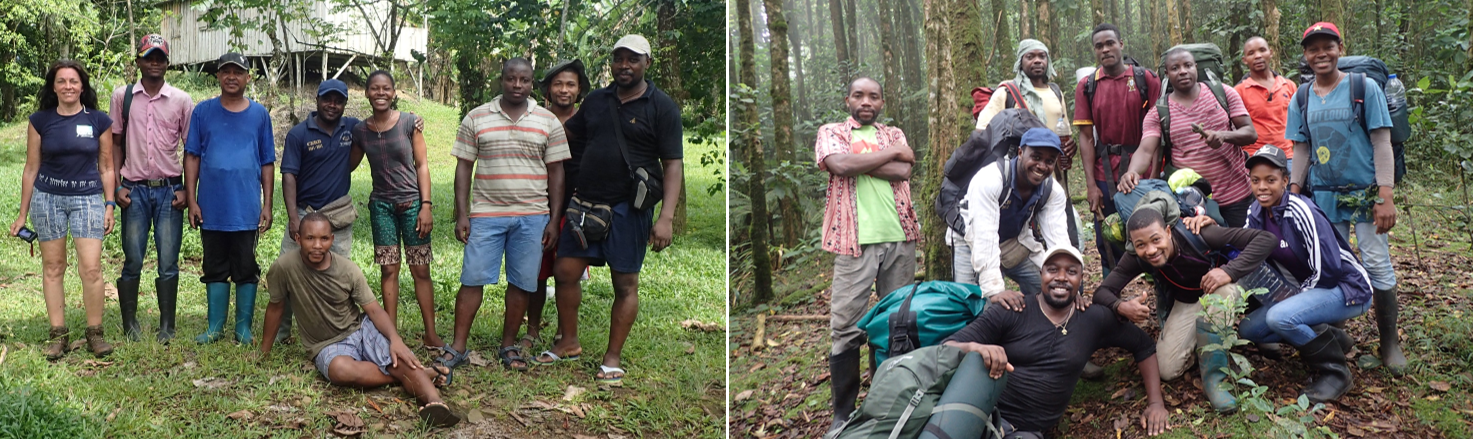
\includegraphics[width=1\linewidth]{D:/MonDossierR/stp_website/static/img/foto_grouped_hor} \caption{Photos of the team during the field campaign in February 2020}\label{fig:unnamed-chunk-2}
\end{figure}

\hypertarget{finding-rare-and-endemic-species}{%
\section{Finding rare and endemic species}\label{finding-rare-and-endemic-species}}

The first expedition in Sao Tomé was, scientifically, a great success. In a period of three weeks, many localities were visited, from the dry North to the wet South and from the coast to the summit of the Pico (2024 m). Thus, most of São Tomé's vegetation types were prospected. Great news from the point of view of conservation, more than 75\% of the island's endemic woody species were found! Some very rare species were rediscovered, including \emph{Balthasaria mannii} (Ternstroemiaceae) and \emph{Psychotria exellii} (Rubiaceae), both restricted to montane forest near the summit of the Pico and not seen for more than 50 years.

\begin{figure}
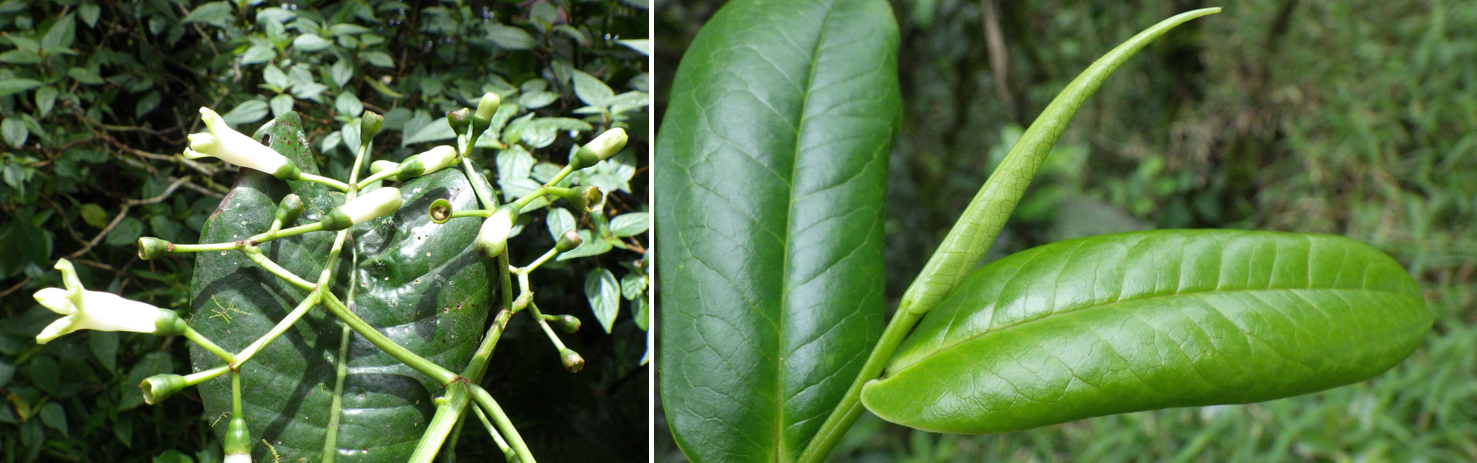
\includegraphics[width=1\linewidth]{D:/MonDossierR/stp_website/static/img/psycho_balthasar} \caption{On the left: *Psychotria exellii*. On the right: *Balthasaria mannii* (photos credit: O. Lachenaud)}\label{fig:unnamed-chunk-3}
\end{figure}

\hypertarget{news-from-pruxedncipe}{%
\section{News from Príncipe}\label{news-from-pruxedncipe}}

The expeditions in Príncipe started in December 2019. With two new staff members, the team performed general collection in four localities, in lowland forest and at the summit of Pico Príncipe (947 m), and also two new transects. Our botanists are focused on collecting good samples of rare and interesting species, found on the previous 24 localities of Príncipe, to identify the species. In the next weeks, we will intensify the surveys, including in the North of the Island.

\begin{figure}
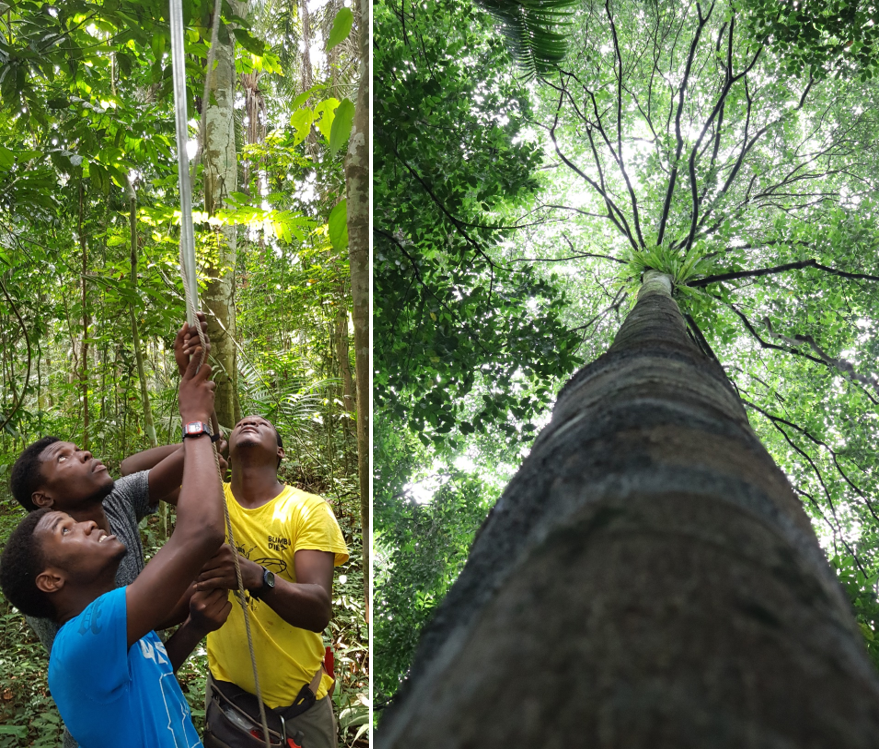
\includegraphics[width=0.8\linewidth]{D:/MonDossierR/stp_website/static/img/principe1} \caption{The challenge to get good material from dominant tree (photos credit: L. Benitez)}\label{fig:unnamed-chunk-4}
\end{figure}

\end{document}
